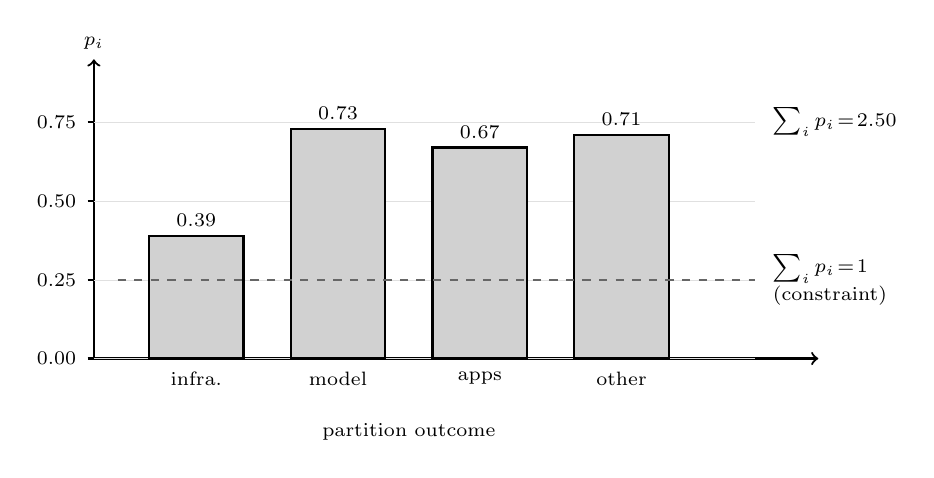
\begin{tikzpicture}
% Axes
\draw[->, thick] (0,0) -- (0,3.8) node[above, font=\scriptsize] {$p_i$};
\draw[->, thick] (0,0) -- (9.2,0);
% Y-axis ticks + faint gridlines
\foreach \y/\lbl in {0/0.00, 1/0.25, 2/0.50, 3/0.75} {
    \draw[black!12, very thin] (0,\y) -- (8.4,\y);
    \draw[thick] (-0.08,\y) -- (0,\y);
    \node[left, font=\scriptsize] at (-0.1,\y) {\lbl};
}
% Bars (data: infra 0.39, model 0.73, apps 0.67, other 0.71; multiply by 4 for height)
\fill[black!18, draw=black, thick] (0.7,0) rectangle (1.9,1.56);
\node[font=\scriptsize] at (1.3,1.56+0.20) {$0.39$};
\fill[black!18, draw=black, thick] (2.5,0) rectangle (3.7,2.92);
\node[font=\scriptsize] at (3.1,2.92+0.20) {$0.73$};
\fill[black!18, draw=black, thick] (4.3,0) rectangle (5.5,2.68);
\node[font=\scriptsize] at (4.9,2.68+0.20) {$0.67$};
\fill[black!18, draw=black, thick] (6.1,0) rectangle (7.3,2.84);
\node[font=\scriptsize] at (6.7,2.84+0.20) {$0.71$};
% X-axis category labels
\node[below, font=\scriptsize] at (1.3,-0.05) {infra.};
\node[below, font=\scriptsize] at (3.1,-0.05) {model};
\node[below, font=\scriptsize] at (4.9,-0.05) {apps};
\node[below, font=\scriptsize] at (6.7,-0.05) {other};
\node[below, font=\scriptsize] at (4.0,-0.7) {partition outcome};
% Dashed constraint line — extends past last bar to give the label clear space on the right
\draw[black!60, dashed, thick] (0.3,1) -- (8.4,1);
% Constraint label — placed in the clear right-side margin, well outside bars
\node[font=\scriptsize, anchor=west, align=left] at (8.5,1) {$\sum_i p_i\!=\!1$\\(constraint)};
% System mass annotation — top right of plot area, in clear space above all bars
\node[font=\scriptsize, anchor=west] at (8.5,3.0) {$\sum_i p_i\!=\!2.50$};
\end{tikzpicture}
